%
%     表紙
%

% 11/21 7:00 nakayama が編集しました。

\documentclass[11pt,b5paper,papersize,dvipdfmx]{jsbook}

\usepackage{vuccaken}
\usepackage{vuccaken2018}

\usepackage[dvipdfmx]{graphicx}
\usepackage{tikz}

% --------------------------------------
\begin{document}

% 表紙
%
\begin{minipage}{0.07\hsize}
  \quad
\end{minipage}
%
\begin{minipage}{0.88\hsize}
  \thispagestyle{empty}
  %
  \begin{center}
    \vspace{-4zw}
    % {\fontsize{90}{0}\selectfont \rm 白 夜}
    
\includegraphics[width=8.5cm]{01img02.png}
  \end{center}
  %
  \begin{flushright}
    \vspace{-7zw}
    {\fontsize{18}{0}\selectfont \bf 第三号  }
  \end{flushright}
  \vspace{2zw}
  %
  \begin{center}
    \vspace{-0.3zw}
    {\fontsize{13}{0}\selectfont \bf 平成三十年度}\\
    \vspace{0.2zw}
    {\fontsize{13}{0}\selectfont \bf 物理科学研究会誌}\\
  \end{center}
  %
  \begin{center}
    \vspace{1zw}
    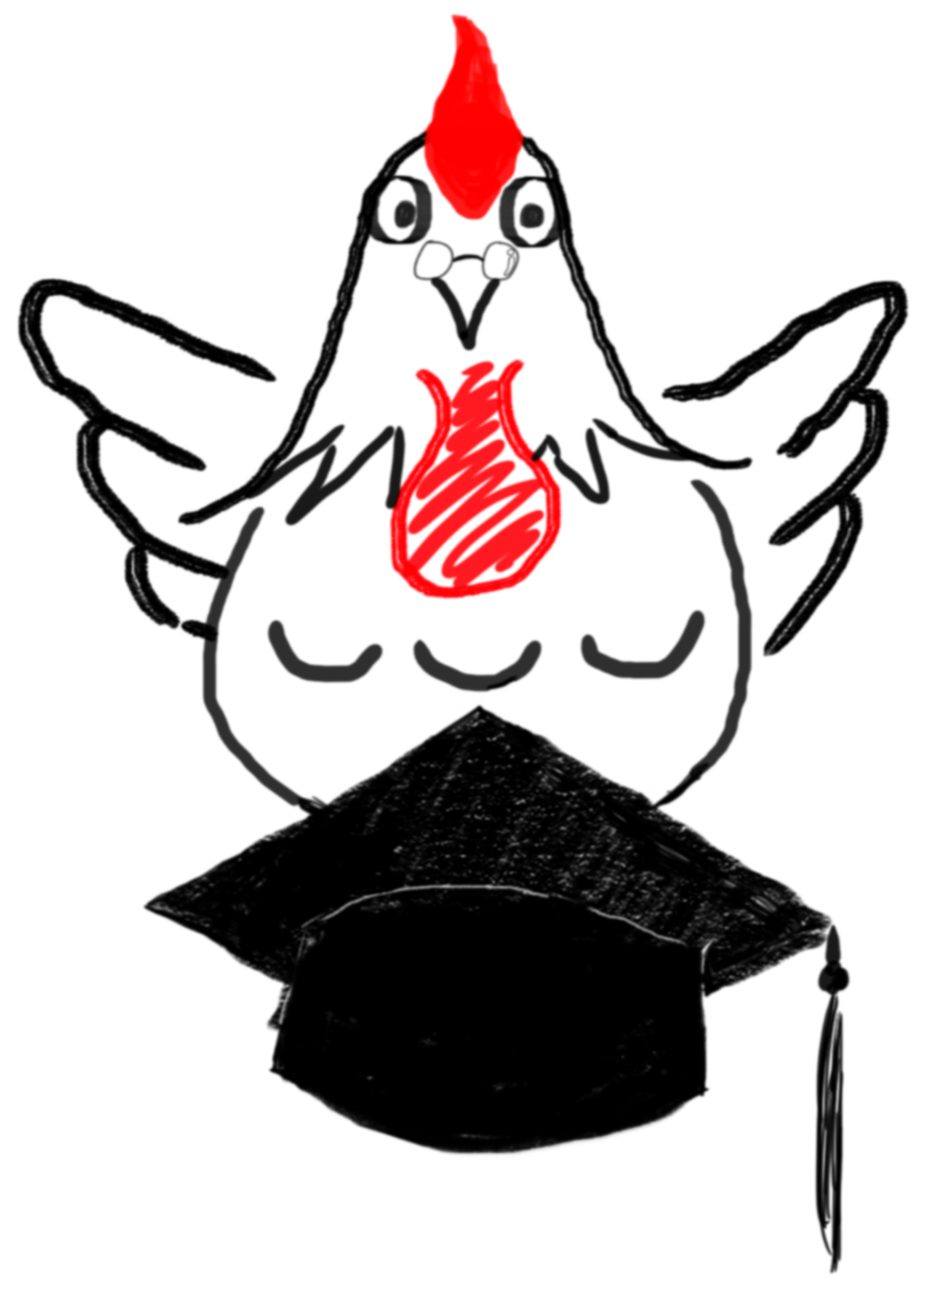
\includegraphics[width=9.5cm]{01img01.png}\\
    \vspace{-2zw}
    {\fontsize{13}{0}\selectfont \gt 学友会学術部}\\
    \vspace{0.2zw}
    {\fontsize{13}{0}\selectfont \gt 立命館大学 物理科学研究会}
  \end{center}
  %
\end{minipage}
%

\newpage 
\quad \thispagestyle{empty}
\newpage

% 中表紙
%
\begin{minipage}{0.07\hsize}
  \quad
\end{minipage}
%
\begin{minipage}{0.88\hsize}
  \tt % font
  \begin{center}
    {\fontsize{50}{0}\selectfont \rm BYAKUYA}\\
    \vspace{3zw}
    {\fontsize{40}{0}\selectfont \rm III}\\
    \vspace{15zw}
    {\fontsize{16}{0}\selectfont BY}\\
    \vspace{0.5zw}
    {\fontsize{18}{0}\selectfont vuccaken}\\
    \vspace{6zw}
    {\fontsize{15}{0}\selectfont 2018.11.25}\\
    \vspace{6zw}
    {\fontsize{15}{0}\selectfont RITSUMEIKAN}\\
    \vspace{3zw}
    {\fontsize{15}{0}\selectfont AT THE SOCIETY}\\
    \vspace{0.5zw}
    {\fontsize{15}{0}\selectfont OF PHYSICAL SCIENCES PRESS}\\
  \end{center}
  \thispagestyle{empty}
\end{minipage}

\newpage 
\quad \thispagestyle{empty}
\newpage





\end{document}
%
% お疲れさまです
%